\usepackage{xeCJK}
\usepackage{tikz,graphicx} 		
\usepackage{booktabs} 			
\usepackage[normalem]{ulem} 	
\usepackage{rotating}  			
\usepackage{cleveref} 			
\usepackage{hyperref} 			
\usepackage[absolute,overlay]{textpos}

\usefonttheme{serif} 
\usepackage[T1]{fontenc}
\usepackage{lmodern}

\hypersetup{pdfpagemode=FullScreen}
\hypersetup{colorlinks=false} 

\setCJKmainfont[BoldFont=SimHei, ItalicFont=KaiTi]{Microsoft YaHei}
\setCJKsansfont{SimHei}
\setCJKmonofont{FangSong}

\makeatletter
\newcommand{\srcsize}{\@setfontsize{\srcsize}{5pt}{5pt}}
\makeatother

\setbeamerfont{title}{family=\sffamily,size=\LARGE} 
\setbeamerfont{subtitle}{family=\sffamily,size=\small}
\setbeamerfont{section in toc}{family=\sffamily,size=\large} 
\setbeamerfont{frametitle}{family=\sffamily}
\setbeamerfont{author}{size=\small}
\setbeamerfont{date}{size=\scriptsize}       

\setbeamertemplate{navigation symbols}{}     

\addtobeamertemplate{title page}{
\tikz[overlay,remember picture] \node[opacity=0.3, at=(current page.center)] {
   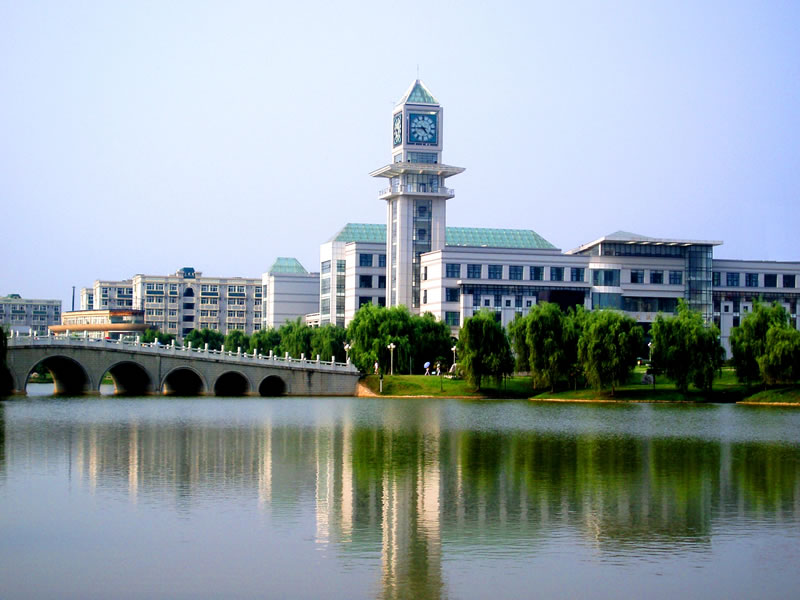
\includegraphics[height=\paperheight,width=\paperwidth]{./img/znufebg.jpg}};
}


%%%%%%%%%%%%%%%%%%%%%%%%%%%%%%%%%%%%%%%%%%%%%%%
\institute{
	{中南财经政法大学} \\
	{\tiny 统计与数学学院} \\
	\smallskip                                          
	\emph {\tiny datalab026a@qq.com}                      
}

% \institute{
%     {Zhongnan University of Economics and Law} \\
%     {\tiny School of Statistics and Mathematics} \\
%     \smallskip                                          
%     \emph {\scriptsize datalab026a@qq.com}                      
% }
%%%%%%%%%%%%%%%%%%%%%%%%%%%%%%%%%%%%%%%%%%%%%%%%%

\setbeamertemplate{title page}[empty]
\setbeamercovered{transparent}



\definecolor{texpurple}{HTML}{522D80}
\definecolor{texorange}{HTML}{F66733}
\definecolor{texblue}{HTML}{2B3856}
\definecolor{antiquewhite}{rgb}{0.98, 0.92, 0.84}
\definecolor{aliceblue}{rgb}{0.94, 0.97, 1.0}
\definecolor{lighttaupe}{rgb}{0.7, 0.55, 0.43}
\definecolor{mediumtaupe}{rgb}{0.4, 0.3, 0.28}
\definecolor{taupe}{rgb}{0.28, 0.24, 0.2}
\definecolor{darktaupe}{rgb}{0.28, 0.24, 0.2}
\definecolor{camouflagegreen}{rgb}{0.47, 0.53, 0.42}

\setbeamercolor{frametitle}{fg=texpurple,bg=white}
\setbeamercolor{title}{fg=texpurple,bg=white}
\setbeamercolor{local structure}{fg=texpurple}
\setbeamercolor{section in toc}{fg=texpurple,bg=white}
\setbeamercolor{section in toc shaded}{fg = texpurple}
\setbeamercolor{subsection in toc}{fg=texblue,bg=white}
\setbeamercolor{item projected}{fg=texpurple,bg=white}
\setbeamertemplate{itemize item}{\color{texpurple}$\bullet$}
\setbeamertemplate{itemize subitem}{\color{texpurple}\scriptsize{$\bullet$}}
\setbeamercolor{caption}{fg = texpurple}
\setbeamercolor{caption name}{fg = texpurple}
\setbeamercolor{normal text}{fg = black}

% block
\newenvironment<>{problock}[1]{%
  \begin{actionenv}#2%
      \def\insertblocktitle{#1}%
      \par%
      \mode<presentation>{%
       \setbeamercolor{block title}{fg=texblue,bg=darktaupe!50!yellow}
       \setbeamercolor{block body}{fg=black,bg=olive!20}
       \setbeamercolor{itemize item}{fg=darktaupe}
       \setbeamercolor{enumerate item}{fg=darktaupe}
       \setbeamertemplate{itemize item}[triangle]
     }%
      \usebeamertemplate{block begin}}
    {\par\usebeamertemplate{block end}\end{actionenv}}

%%%%%%%%%%%%%%%%%%%%%%%%%%%%%%%%%%%%%%%%%%%
\useoutertheme[right,height=0pt,width=0.12\paperwidth]{sidebar}
\setbeamertemplate{sidebar canvas right}[horizontal shading][left=aliceblue!80!camouflagegreen,right=white] 
\setbeamercolor{title in sidebar}{fg=taupe}  
\setbeamercolor{author in sidebar}{fg=taupe}
\setbeamercolor{section in sidebar}{fg=lighttaupe}
\setbeamercolor{section in sidebar shaded}{fg=darktaupe}
\setbeamercolor{subsection in sidebar}{fg=lighttaupe}
\setbeamercolor{subsection in sidebar shaded}{fg=darktaupe}
\setbeamerfont{title in sidebar}{family=\sffamily} 
\setbeamerfont{author in sidebar}{family=\sffamily} 
\setbeamerfont{section in sidebar}{family=\sffamily} 
\setbeamerfont{subsection in sidebar}{family=\sffamily} 
% \setbeamerfont{title in sidebar}{size=\fontsize{5}{5}\selectfont}
% \setbeamerfont{author in sidebar}{size=\fontsize{3}{3}\selectfont}
% \setbeamerfont{section in sidebar}{size=\fontsize{5}{5}\selectfont}
% \setbeamerfont{subsection in sidebar}{size=\fontsize{4}{4}\selectfont}
\usetheme[hideothersubsections]{}


\newlength\imageheight
\settoheight\imageheight{
\includegraphics[width=0.11\paperwidth]{./img/znufe.png}}

\makeatletter
\setbeamertemplate{sidebar \beamer@sidebarside}
  {
    \vspace*{\imageheight}
    \beamer@tempdim=\beamer@sidebarwidth%
    \advance\beamer@tempdim by -6pt%
    {\usebeamerfont{title in sidebar}%
        \vskip1.5em%
        \hskip3pt%
        \usebeamercolor[fg]{title in sidebar}%
        \insertshorttitle[width=\beamer@tempdim,center,respectlinebreaks]\par%
        \vskip1.25em%
    }%
    {%
        \hskip3pt%
        \usebeamercolor[fg]{author in sidebar}%
        \usebeamerfont{author in sidebar}%
        \insertshortauthor[width=\beamer@tempdim,center,respectlinebreaks]\par%
        \vskip1.25em%
    }%
    \insertverticalnavigation{\beamer@sidebarwidth}%
    \vfill
    \ifx\beamer@sidebarside\beamer@lefttext%
    \else%
    \usebeamercolor{normal text}%
    \llap{\usebeamertemplate***{navigation symbols}\hskip0.1cm}%
    \vskip2pt%
    \fi%
  }%
\setbeamertemplate{section in sidebar}%{sidebar theme}
{%
  \vbox{%
    \vskip1ex%
    \beamer@sidebarformat{3pt}{section in sidebar}{\insertsectionheadnumber
~\insertsectionhead}%
  }%
}
\setbeamertemplate{section in sidebar shaded}%{sidebar theme}
{%
  \vbox{%
    \vskip1ex%
    \beamer@sidebarformat{3pt}{section in sidebar shaded}{\insertsectionheadnumber
~\insertsectionhead}%
  }%
}

\makeatletter
\addtobeamertemplate{sidebar right}{}{%
    \begin{tikzpicture}[remember picture,overlay] % 
        \node[anchor=north east,yshift=2pt] at (current page.north east) {
\includegraphics[width=0.11\paperwidth]{./img/znufe.png}};
    \end{tikzpicture}
    }
\makeatother


\setbeamertemplate{footline}{% footline add page number
\hfill\usebeamertemplate***{navigation symbols}
\hspace{1cm}\insertframenumber{}/\inserttotalframenumber}

\setbeamercolor{footline}{fg=texpurple}
\setbeamerfont{footline}{series=\bfseries}

\setbeamertemplate{caption}{%
\begin{beamercolorbox}[wd=\paperwidth, dp=0.5ex, sep=0.2ex, center]{block body}\insertcaption%
\end{beamercolorbox}%
}

\newcommand\FootText[1]{
  \begin{textblock*}{\textwidth}(0pt,\textheight)\raggedright #1 \hspace{20pt}\end{textblock*}}


\AtBeginPart{}

\AtBeginSection[]{
  \begin{frame}[c]
    \begin{center}
      \setbeamerfont{section in toc}{family=\sffamily,size=\LARGE} 
      \tableofcontents[sectionstyle=show/hide,subsectionstyle=hide/show/hide]
    \end{center}
  \end{frame}
}
\AtBeginSubsection{}
\AtBeginSubsubsection{}
\setlength{\emergencystretch}{0em}
\setlength{\parskip}{0pt}